\section*{CHAPTER 6. RESULTS AND DISCUSSION}
\addcontentsline{toc}{section}{\numberline{}CHAPTER 6. RESULTS AND DISCUSSION}

\setcounter{section}{6}
\setcounter{subsection}{0}
\setcounter{figure}{0}
\setcounter{table}{0}

\subsection{System Configuration and Simulation Scenarios}

The physical architecture of the proposed energy management system comprises one Main Grid (MG0) and four interconnected Microgrids (MG1, MG2, MG3, and MG4). These Microgrids (MGs) form a Peer-to-Peer (P2P) trading network, establishing a cooperative environment that facilitates active power exchange. This P2P interconnection is specifically designed to enhance system resilience, allowing the MGs to support one another through internal power transfers, especially when isolated from the Main Grid. To ensure grid stability and respect physical tie-line capacities, the power exchange between any connected MGs is strictly constrained within a trading limit of $\pm 1.5$ MW (1.5 pu, given a system base power of 1 MVA).

The physical network topology (Figure \ref{fig:p2p_topology}) integrates four distinct MGs:

\begin{figure}[htbp]
    \centering
    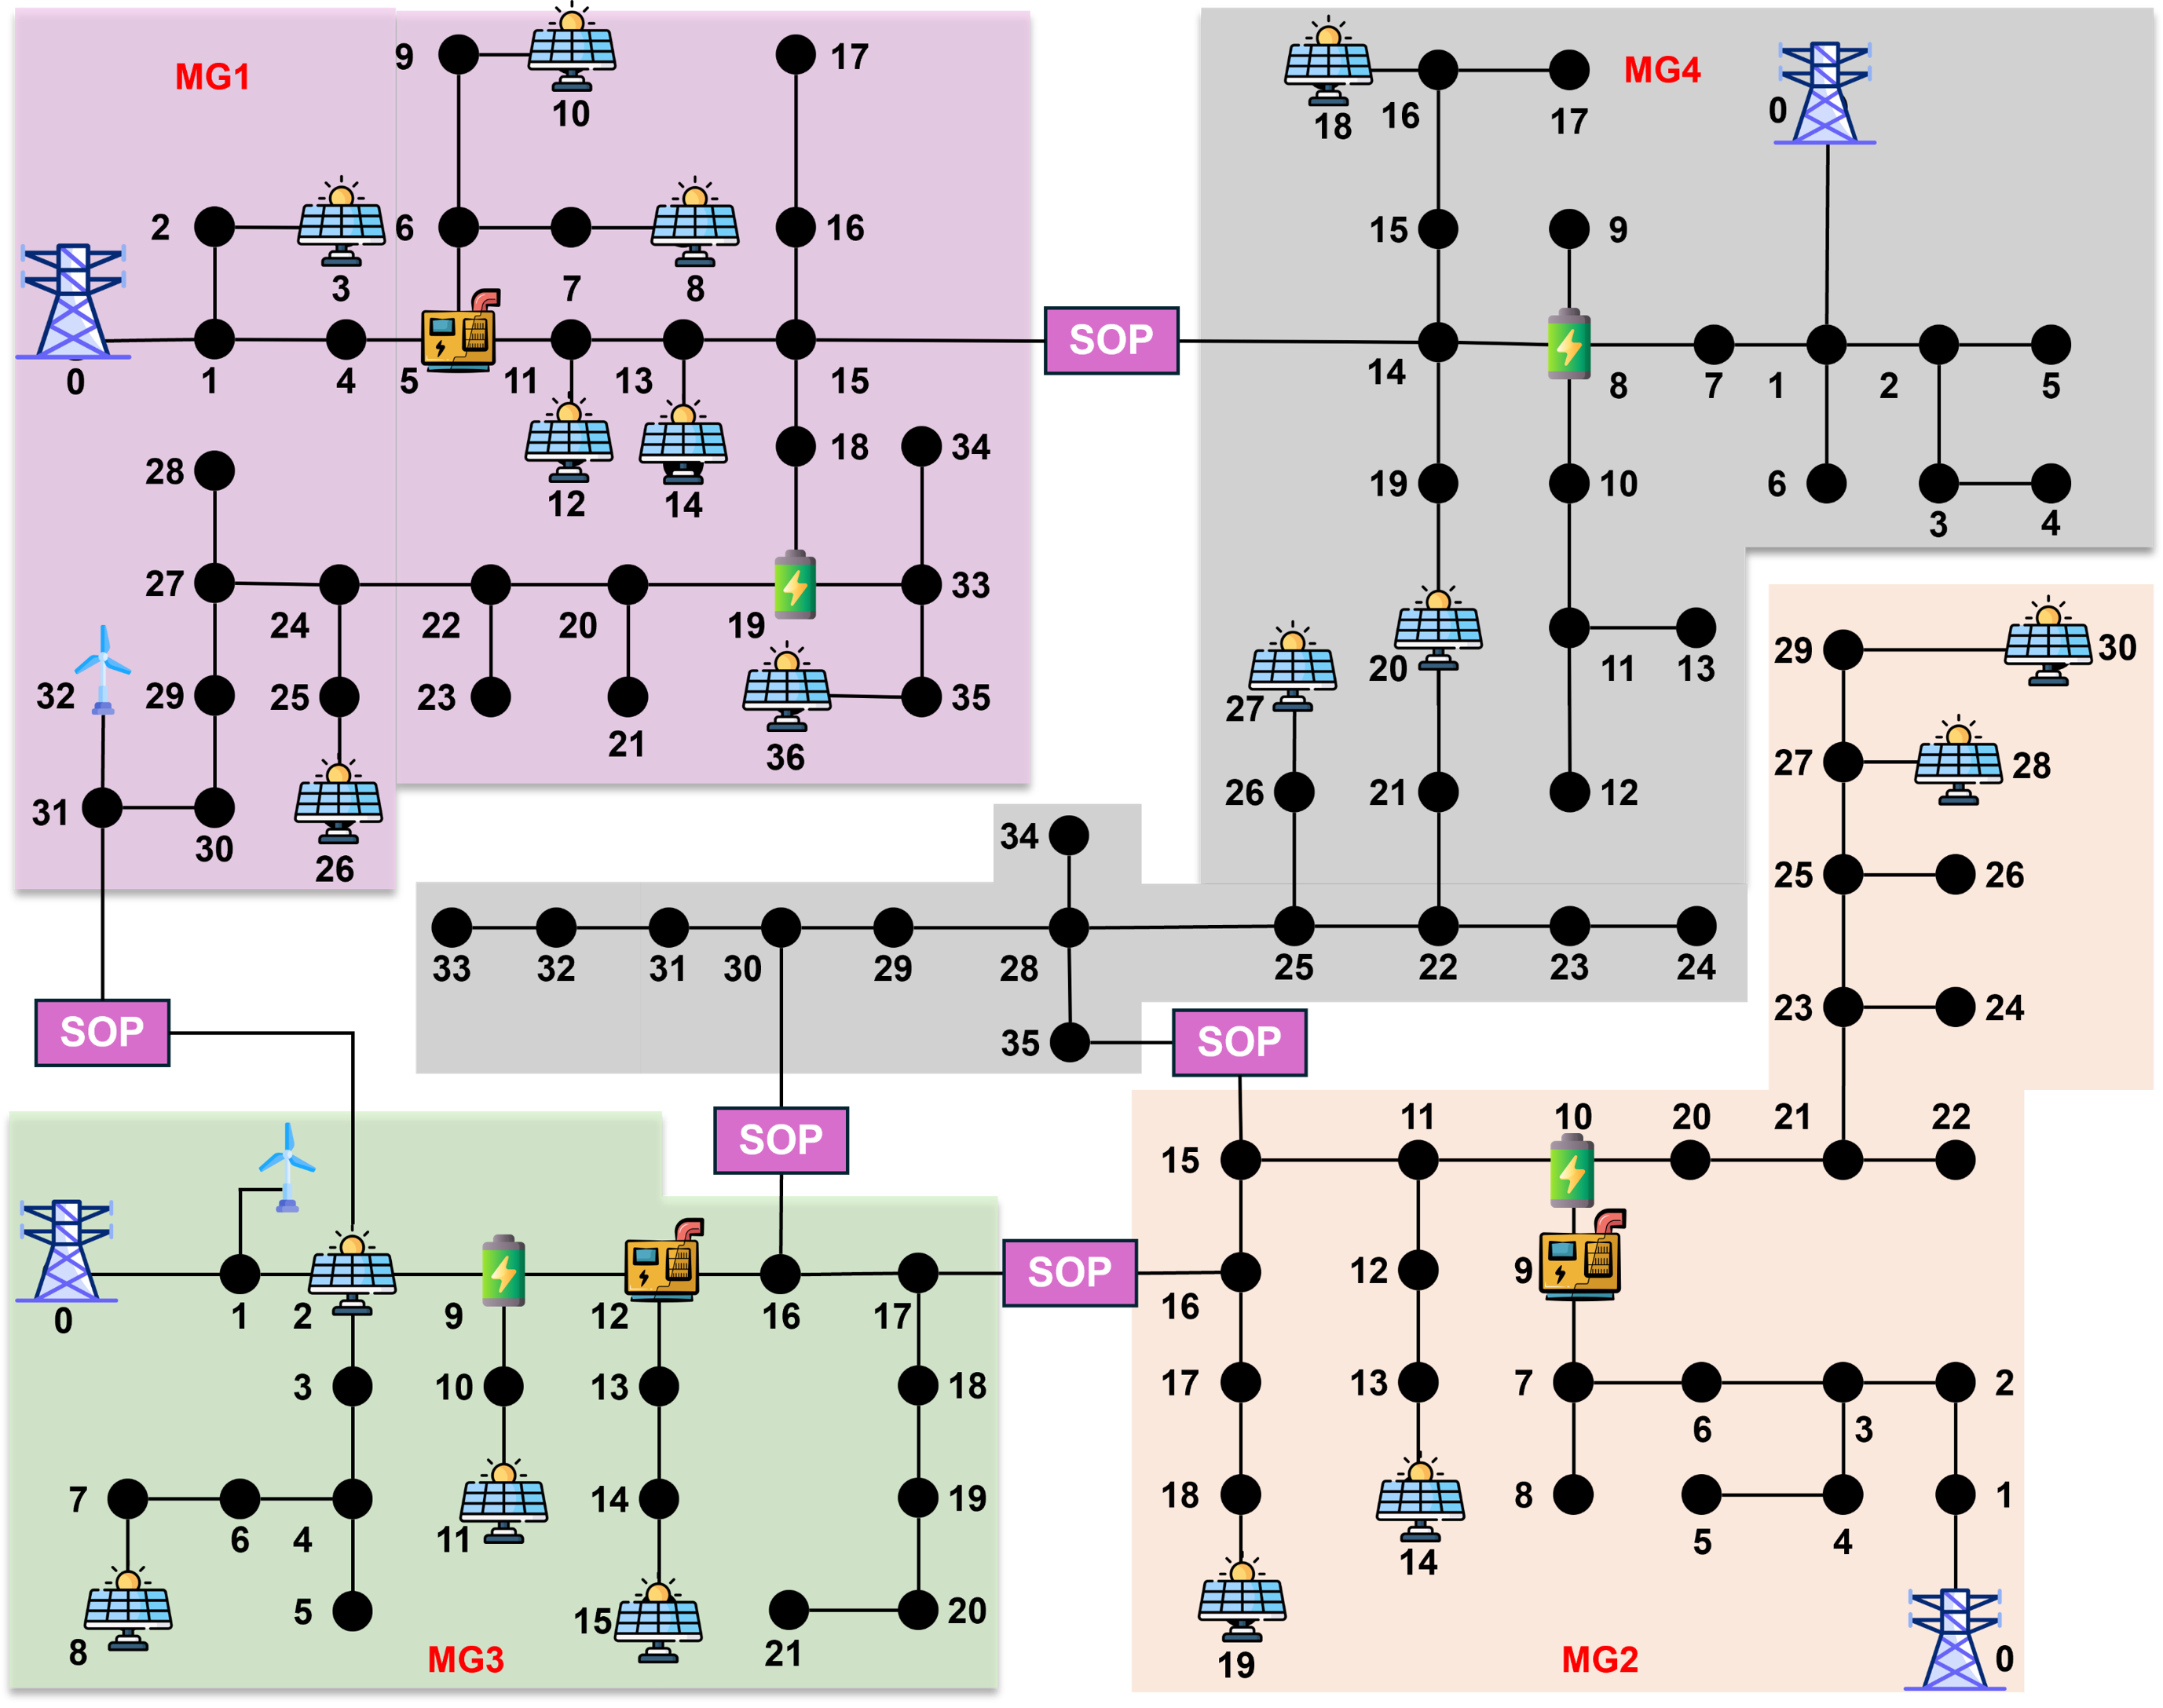
\includegraphics[width=\textwidth]{chapters/Imagine/ALL_MG_fixed.png}
    \caption{Peer-to-Peer interconnection topology of the multi-microgrid system.}
    \label{fig:p2p_topology}
\end{figure}

\begin{itemize}
    \item \textbf{Microgrid 1 (MG1):} 36-node network with diverse generation (PV, WT, BESS, DG). Maintains physical P2P tie-lines with MG3 and MG4.
    
    \item \textbf{Microgrid 2 (MG2):} 30-node radial solar-only network with BESS and DG. Directly connected to MG3 and MG4.
    
    \item \textbf{Microgrid 3 (MG3):} 21-node network with excess generation capabilities. Interconnected with MG1, MG2, and MG4.
    
    \item \textbf{Microgrid 4 (MG4):} 35-node complex with high consumption and PV capacity. Interconnected with MG1, MG2, and MG3.
\end{itemize}

\subsubsection{System Parameters and DER Allocation}
To ensure the mathematical models accurately reflect physical distribution networks, the specific allocation of Distributed Energy Resources (DERs) across the four microgrids---as structurally depicted in Figure \ref{fig:p2p_topology}---is systematically summarized in Table \ref{tab:der_placement}.

\begin{table}[htbp]
    \centering
    \caption{Placement of Distributed Energy Resources across Microgrids}
    \label{tab:der_placement}
    \resizebox{0.9\textwidth}{!}{%
    \begin{tabular}{lccccc}
        \toprule
        \textbf{Microgrid} & \textbf{Total Nodes} & \textbf{PV Nodes} & \textbf{WT Nodes} & \textbf{BESS Node} & \textbf{DG Node} \\
        \midrule
        \textbf{MG1} & 36 & 3, 10, 12, 14, 26, 36 & 32 & 19 & 5 \\
        \textbf{MG2} & 30 & 14, 19, 28, 30 & - & 20 & 10 \\
        \textbf{MG3} & 21 & 2, 8, 11, 15 & 1 & 12 & 9 \\
        \textbf{MG4} & 35 & 18, 20, 27, 29 & - & 8 & 22 \\
        \bottomrule
    \end{tabular}%
    }
\end{table}

Furthermore, the critical technical and economic parameters governing the operational costs of the Dispatchable Generators (DG) and Battery Energy Storage Systems (BESS) are identically configured across all deployed units. These parameters form the foundational cost coefficients for the objective function and are summarized in Table \ref{tab:dg_bess_params}.

\begin{table}[htbp]
    \centering
    \caption{Technical and Economic Parameters of DG and BESS}
    \label{tab:dg_bess_params}
    \resizebox{0.95\textwidth}{!}{%
    \begin{tabular}{llc}
        \toprule
        \textbf{Component} & \textbf{Parameter} & \textbf{Value (pu / nominal)} \\
        \midrule
        \textbf{Dispatchable} & Minimum / Maximum Output ($P_{DG}^{min}$ / $P_{DG}^{max}$) & $0.2 / 1.3$ \\
        \textbf{Generator} & Ramp Rate Limit ($R_{DG}$) & $1.0$ \\
        \textbf{(DG)} & Minimum Up/Down Time ($T_{up}^{DG}$, $T_{down}^{DG}$) & $2$ hours \\
        & Fixed Cost Coefficient ($\alpha_{DG}$) & $700$ \\
        & Linear Cost Coefficient ($\beta_{DG}$) & $16.06$ \\
        & Quadratic Cost Coefficient ($\gamma_{DG}$) & $0.002$ \\
        & O\&M Cost Coefficient ($\kappa_{DG}$) & $1.258$ \\
        & Hot / Cold Start Cost ($C_{start,DG}$) & $660 / 1120$ \\
        \midrule
        \textbf{Battery Energy} & Energy Capacity ($E_{BESS}$) & $1.5$ \\
        \textbf{Storage} & Maximum Power ($P_{BESS}^{max}$) & $0.75$ \\
        \textbf{(BESS)} & Charge/Discharge Efficiency ($\eta_{BESS}$) & $0.90$ \\
        & $SOC^{min}$ / $SOC^{max}$ / $SOC^{ini}$ & $0.20 / 0.95 / 0.40$ \\
        & Degradation Cost ($C_{BESS}$) & $7.125$ \\
        \bottomrule
    \end{tabular}%
    }
\end{table}

\subsubsection{Simulation Scenarios and Fault Configurations}
To rigorously evaluate the resilience of the proposed energy management system, a compounded emergency fault is simulated based on realistic parameter bounds derived from the system's generation profiles and limits. The simulated emergency event is characterized by the simultaneous occurrence of two severe failures:
\begin{itemize}
    \item \textbf{Main Grid Loss:} A complete disconnection from the utility grid (MG0) occurs between $t=9$ and $t=15$, forcing the entire multi-microgrid network into islanded operation.
    \item \textbf{PV Generation Loss:} A severe drop in solar power generation affects all Photovoltaic units between $t=11$ and $t=15$, representing an extreme weather anomaly.
\end{itemize}

Under these harsh operating conditions, three distinct comparison scenarios are defined to evaluate the proposed framework:
\begin{itemize}
    \item \textbf{Base Fault:} Isolated operation without P2P energy sharing during the emergency.
    \item \textbf{Perfect Foresight:} Ideal centralized approach with perfect prediction of the entire horizon.
    \item \textbf{Current Method (MPC):} The proposed decentralized rolling-horizon MPC with limited foresight.
\end{itemize}

\subsection{Macro-Economic Assessment and Load Protection}

This section evaluates the quantitative performance of the three defined simulation models based on true economic outcomes and global optimality. To ensure a rigorous comparison, boundary conditions for the Battery Energy Storage Systems (BESS) are strictly enforced, mandating that the State of Charge (SOC) at the end of the simulation horizon equals the initial SOC ($SOC_{24} = SOC_{0}$). Furthermore, algorithmic penalties (such as SOC or cross-penalties) are excluded to formulate the True Economic Cost, which is defined strictly by pure fuel expenses and load shedding compensation. 

Table \ref{tab:benchmark_stage1} summarizes the macro-economic benchmark results for the three scenarios.

\begin{table}[htbp]
    \centering
    \caption{Macro-Economic Benchmark of Simulation Models}
    \label{tab:benchmark_stage1}
    \resizebox{\textwidth}{!}{%
    \begin{tabular}{lccccc}
        \toprule
        \textbf{Model} & \textbf{Pure Cost (cents)} & \textbf{Pure Gap} & \textbf{True Eco Cost (cents)} & \textbf{Eco Gap} & \textbf{Shedding (MWh)} \\
        \midrule
        \textbf{Base Fault} & 179,695.79 & 5.02\% & 1,722,260.04 & 272.41\% & 15.4260 \\
        \textbf{Perfect Foresight} & 171,100.35 & Baseline & 462,462.02 & Baseline & 2.9138 \\
        \textbf{Current Method} & 179,007.53 & 4.62\% & 470,294.90 & 1.69\% & 2.9129 \\
        \bottomrule
    \end{tabular}%
    }
    
    \vspace{1ex}
    \small \textit{Note: The minute disparity in load shedding between Perfect Foresight (2.9138 MWh) and the Current Method (2.9129 MWh) is mathematically negligible and stems exclusively from numerical solver convergence tolerances rather than algorithmic inferiority.}
\end{table}

The benchmark analysis, visually supported by Figure \ref{fig:cost_vs_shedding}, reveals three core signature contributions of the proposed decentralized Model Predictive Control (MPC) framework:
\begin{figure}[htbp]
    \centering
    
\includegraphics[width=0.85\textwidth]{"Transfer folder/Result_data/report_result/stage_1/Stage1_Cost_vs_Shedding.png"}
    \caption{Macro-economic comparison demonstrating the true economic cost versus total load shedding.}
    \label{fig:cost_vs_shedding}
\end{figure}

\subsubsection{100\% Critical Load Protected}
The primary objective during emergency operation is the minimization of unserved energy, specifically shielding critical infrastructure. Under the isolated Base Fault scenario, the lack of cooperative Peer-to-Peer (P2P) sharing forces the system to shed $15.4260$ MWh of load due to localized power depletion. Implementing the decentralized MPC drastically reduces this shedding to merely $2.9129$ MWh, closely mirroring the ideal performance of the Perfect Foresight model ($2.9138$ MWh). 

Mathematically, the financial data confirms the complete protection of critical loads. The shedding compensation incurred by the MPC is the difference between its true economic cost and pure cost ($470,294.90 - 179,007.53 = 291,287.37$ cents). Dividing this penalty by the curtailed energy ($2.9129$ MWh) yields an exact compensation rate of $100,000$ cents/MWh. This matches the Value of Lost Load (VOLL) assigned strictly to Normal Loads. Consequently, this demonstrates that all curtailed power was exclusively non-essential, confirming that the framework successfully protected 100\% of the Critical Load during severe compounded outages.

\subsubsection{The Denominator Effect: Shifting the Optimality Gap}
Although the proposed MPC operates under a decentralized architecture with a limited rolling horizon, its generation dispatch expenses (Pure Cost) stand at $179,007.53$ cents, maintaining an Optimality Gap of $4.62\%$ relative to the centralized Perfect Foresight benchmark ($171,100.35$ cents). 

More importantly, when evaluating the overarching system resilience through the \textit{True Economic Gap}, the disparity collapses to a mere $1.69\%$. This performance gap highlights a crucial operational phenomenon: The short-sightedness of the rolling horizon slightly compromises the optimal economic dispatch of generation resources, but it fundamentally does not degrade the system's energy security capability. This behavior is mathematically driven by the objective function's weighting. The penalty factor for load shedding (Value of Lost Load, VOLL = 100,000 cents/MWh) is orders of magnitude higher than the marginal cost of standard generation ($\sim 16$ cents). Therefore, even with only a 1-hour look-ahead window, the objective gradient heavily prioritizes immediate BESS discharge and P2P sharing to avert shedding at all costs. The MPC's myopic nature only leads to suboptimal fuel purchasing schedules, but it will never elect to shed load unless physical capacities are entirely exhausted.

\begin{figure}[htbp]
    \centering
    
\includegraphics[width=0.85\textwidth]{"Transfer folder/Result_data/report_result/stage_1/Stage1_Energy_Mix.png"}
    \caption{Energy mix distribution across the multi-microgrid system over a 24-hour horizon.}
    \label{fig:energy_mix}
\end{figure}

\subsubsection{Resilience with Synergistic Negative Premium}
Cross-examining the Base Fault and MPC scenarios uncovers the synergistic benefits of the P2P architecture. Typically, enhancing system resilience to supply an additional $12.51$ MWh (the difference in shedding between Base Fault and MPC) requires a Resilience Premium by ramping up expensive localized generation. However, the MPC achieves this while actually lowering the total generation cost ($179,007.53$ cents) compared to the isolated Base Fault ($179,695.79$ cents).

This remarkable capability to provide resilience at a Negative Premium stems from unblocking stranded renewable energy. As illustrated in Figure \ref{fig:energy_mix}, excess photovoltaic and wind generation from healthy nodes—which would otherwise be curtailed under isolated conditions—is effectively routed to deficit regions. The P2P network, dynamically regulated by the MPC, forms a symbiotic ecosystem that simultaneously saves critical loads and optimizes overall fuel expenditure.

\subsection{Micro-System Dynamics}



\begin{figure}[H]
    \centering
    \begin{subfigure}[b]{0.48\textwidth} 
\includegraphics[width=\textwidth]{{Transfer folder/Result_data/report_result/stage_2/SOC_Comparison_MG1.png}} \caption{MG1} \end{subfigure}\hfill
    \begin{subfigure}[b]{0.48\textwidth} 
\includegraphics[width=\textwidth]{{Transfer folder/Result_data/report_result/stage_2/SOC_Comparison_MG2.png}} \caption{MG2} \end{subfigure}
    \vspace{0.3cm}
    \begin{subfigure}[b]{0.48\textwidth} 
\includegraphics[width=\textwidth]{{Transfer folder/Result_data/report_result/stage_2/SOC_Comparison_MG3.png}} \caption{MG3} \end{subfigure}\hfill
    \begin{subfigure}[b]{0.48\textwidth} 
\includegraphics[width=\textwidth]{{Transfer folder/Result_data/report_result/stage_2/SOC_Comparison_MG4.png}} \caption{MG4} \end{subfigure}
    \caption{BESS State-of-Charge (SOC) Comparison.}
    \label{fig:soc_comparison}
\end{figure}

\subsubsection{Base Fault: The Vulnerability of Isolation}
The Base Fault scenario simulates an isolated operation where Peer-to-Peer (P2P) trading is strictly prohibited. Even though this baseline model is theoretically configured with knowledge of the impending fault, its inability to dynamically share power across the network severely restricts system operability. As observed in the Active Power profiles (Figure \ref{fig:base_fault_active_power}), each MG is strictly confined to its local generation. When the dual contingency strikes, the isolated microgrids---particularly the heavily loaded MG1 and the densely populated MG4---rapidly exhaust their local BESS capacities. The SOC Comparison curves (Figure \ref{fig:soc_comparison}) for MG1 and MG4 drop to their absolute minimum limits as the batteries are drained in an effort to sustain local demands. Without spatial coordination, surplus energy in healthy regions remains stranded, leading to massive localized power depletion and forcing the system to shed $15.4260$ MWh of load.

\begin{figure}[H]
    \centering
    \begin{subfigure}[b]{0.48\textwidth} 
\includegraphics[width=\textwidth]{{Transfer folder/Result_data/report_result/stage_2/base_fault_Active_Power_MG1.png}} \caption{MG1} \end{subfigure}\hfill
    \begin{subfigure}[b]{0.48\textwidth} 
\includegraphics[width=\textwidth]{{Transfer folder/Result_data/report_result/stage_2/base_fault_Active_Power_MG2.png}} \caption{MG2} \end{subfigure}
    \vspace{0.3cm}
    \begin{subfigure}[b]{0.48\textwidth} 
\includegraphics[width=\textwidth]{{Transfer folder/Result_data/report_result/stage_2/base_fault_Active_Power_MG3.png}} \caption{MG3} \end{subfigure}\hfill
    \begin{subfigure}[b]{0.48\textwidth} 
\includegraphics[width=\textwidth]{{Transfer folder/Result_data/report_result/stage_2/base_fault_Active_Power_MG4.png}} \caption{MG4} \end{subfigure}
    \caption{Active Power Flow - Base Fault Scenario.}
    \label{fig:base_fault_active_power}
\end{figure}

\subsubsection{Perfect Foresight: The Advantage of Absolute Knowledge}
The Perfect Foresight (PF) model operates with absolute knowledge of the entire 24-hour horizon. This predictive supremacy manifests as a highly proactive energy management strategy, clearly visible in the SOC Comparison charts (Figure \ref{fig:soc_comparison}). Rather than passively maintaining charge before the emergency, the PF model exhibits a sophisticated "Anticipatory Discharge" behavior. Specifically, at $t=8$, right before the main grid fault occurs, the PF model intentionally discharges the BESS down to its minimum limit ($SOC = 0.2$). This is not a random action, but a strategic clearing of energy headroom. Knowing that the main grid will fail at $t=9$, but local solar generation will still be abundant during $t=9$ and $t=10$ before the PV outage at $t=11$, the algorithm makes room to aggressively capture this free solar energy. Consequently, it rapidly charges the BESS from $0.2$ to near-maximum capacity ($\sim 0.95$) within those two hours.

During the darkest fault hours ($t=11$ to $t=15$), this strategically stored energy is deployed. By optimally manipulating its energy boundaries and clearing headroom based on future knowledge, the PF model maximizes renewable energy utilization while avoiding unnecessary grid purchases. This flawless temporal energy shifting minimizes the need for urgent power transfers, resulting in highly stable Active Power flows (Figure \ref{fig:pf_active_power}) and achieving the theoretical minimum operational cost.

\begin{figure}[htbp]
    \centering
    \begin{subfigure}[b]{0.48\textwidth} 
\includegraphics[width=\textwidth]{{Transfer folder/Result_data/report_result/stage_2/foresight_model_Active_Power_MG1.png}} \caption{MG1} \end{subfigure}\hfill
    \begin{subfigure}[b]{0.48\textwidth} 
\includegraphics[width=\textwidth]{{Transfer folder/Result_data/report_result/stage_2/foresight_model_Active_Power_MG2.png}} \caption{MG2} \end{subfigure}
    \vspace{0.3cm}
    \begin{subfigure}[b]{0.48\textwidth} 
\includegraphics[width=\textwidth]{{Transfer folder/Result_data/report_result/stage_2/foresight_model_Active_Power_MG3.png}} \caption{MG3} \end{subfigure}\hfill
    \begin{subfigure}[b]{0.48\textwidth} 
\includegraphics[width=\textwidth]{{Transfer folder/Result_data/report_result/stage_2/foresight_model_Active_Power_MG4.png}} \caption{MG4} \end{subfigure}
    \caption{Active Power Flow - Perfect Foresight Model.}
    \label{fig:pf_active_power}
\end{figure}

\subsubsection{Proposed MPC: The Hoarding Syndrome and P2P Rescue}
In stark contrast, the proposed decentralized Model Predictive Control (MPC) operates under a limited rolling horizon, rendering it entirely blind to the true duration and severity of the impending emergency. This lack of long-term visibility fundamentally alters the battery dispatch behavior. Prior to the fault, the MPC maintains flat, standard economic SOC profiles, failing to proactively pre-charge. More importantly, when the fault suddenly hits at $t=9$, the MPC adopts a conservative energy retention strategy. Because it cannot foresee the end of the outage, the algorithm becomes highly reluctant to fully discharge its limited BESS reserves, reserving them against future uncertainties. As seen in the SOC Comparison graphs (Figure \ref{fig:soc_comparison}), rather than smoothly depleting the batteries like the Perfect Foresight model, the MPC significantly restricts its BESS discharge rates. 

To manage the contingency and compensate for this conservative discharge approach, the MPC is forced to rely almost exclusively on the P2P network as a primary support mechanism. The Active Power flow graphs (Figure \ref{fig:mpc_active_power}) illustrate this highly dynamic and spatially shifted support operation. During the initial phase of the grid isolation ($t=9, t=10$), the system relies heavily on two primary supporting units: MG2 (leveraging its dense solar capacity) and MG3 (benefiting from its light industrial load). These two microgrids actively export significant amounts of surplus power through the tie-lines to sustain the power-deficient microgrids, MG1 and MG4. 

However, when the compounded severe PV loss strikes at $t=11$, the entire internal power flow topology undergoes a violent restructuring. MG2, suddenly stripped of its primary solar resource, rapidly depletes its limited local capacities and undergoes a complete "Parasitic Shift," transforming into a massive power sink. Concurrently, MG1 (which possesses robust wind and PV generation) and MG3 emerge as the dual powerhouses of the network. For the remainder of the fault ($t=11$ to $t=15$), MG1 and MG3 generate massive surpluses and aggressively export power to rescue the deficit regions. 

Within this extreme power routing, MG4 is forced into the highly disadvantageous role of a "Transit Corridor" (Wheeling Hub). It imports massive amounts of active power from MG1 and MG3, only to wheel a significant portion of it directly to the collapsed MG2. This creates a profound operational irony: MG4 is forced to execute active load shedding NOT because it lacks access to active power (P), but because the sheer volume of power flowing through its distribution feeders to save MG2 induces massive currents ($I$). These transit currents exponentially inflate the local reactive power losses ($I^2X$), dragging down MG4's voltage profile and forcing it to shed its own local loads just to maintain the physical viability of the transmission path. MG4 essentially sacrifices its own normal loads to serve as a lifeline for MG2.

This intense reliance on spatial P2P sharing causes highly volatile spikes in active power exchange. However, it is precisely this reactive, aggressive coordination that unblocks stranded renewable energy from the surviving units (MG1 and MG3), routing it to where it is needed most. Consequently, the MPC brilliantly manages to protect 100\% of the critical loads and achieve a synergistic Negative Premium, turning its short-sighted temporal limitation into a profound spatial advantage.
\begin{figure}[htbp]
    \centering
    \begin{subfigure}[b]{0.48\textwidth} 
\includegraphics[width=\textwidth]{{Transfer folder/Result_data/report_result/stage_2/current_method_Active_Power_MG1.png}} \caption{MG1} \end{subfigure}\hfill
    \begin{subfigure}[b]{0.48\textwidth} 
\includegraphics[width=\textwidth]{{Transfer folder/Result_data/report_result/stage_2/current_method_Active_Power_MG2.png}} \caption{MG2} \end{subfigure}
    \vspace{0.3cm}
    \begin{subfigure}[b]{0.48\textwidth} 
\includegraphics[width=\textwidth]{{Transfer folder/Result_data/report_result/stage_2/current_method_Active_Power_MG3.png}} \caption{MG3} \end{subfigure}\hfill
    \begin{subfigure}[b]{0.48\textwidth} 
\includegraphics[width=\textwidth]{{Transfer folder/Result_data/report_result/stage_2/current_method_Active_Power_MG4.png}} \caption{MG4} \end{subfigure}
    \caption{Active Power Flow - Proposed MPC Method.}
    \label{fig:mpc_active_power}
\end{figure}


\subsection{Node-Level Voltage and Reactive Power}

This section analyzes the local power quality, voltage stability, and load shedding behaviors at the nodal level to evaluate the physical feasibility of the proposed framework.

The load shedding profiles, depicted in Figure \ref{fig:load_shedding}, demonstrate the prioritization mechanism of the energy management algorithm. Critical load shedding remains at zero across all four microgrids throughout the simulated horizon. During the compounded fault period, load curtailment is confined entirely to normal loads within Microgrid 4 (MG4), which suffers from the most severe local deficit due to its dense load and massive PV generation loss. Furthermore, a deeper spatial analysis within MG4 reveals that the curtailed loads are predominantly located at the downstream, end-of-line nodes. Because these remote nodes naturally experience the most severe voltage drops along the radial feeders, shedding their normal loads is mathematically the most effective way for the AC-OPF algorithm to relieve network congestion and stabilize local voltage profiles. This behavior confirms the system's capability to maintain supply to critical infrastructure while optimally isolating the inevitable sacrifices to the most electrically vulnerable locations.

\begin{figure}[htbp]
    \centering
    
\includegraphics[width=0.75\textwidth]{{Transfer folder/Result_data/report_result/stage_3/Load_Shedding_MG4.png}}
    \caption{Load Shedding Profile (Confined exclusively to MG4).}
    \label{fig:load_shedding}
\end{figure}

Furthermore, an AC-OPF analysis of Microgrid 4 (MG4) reveals a critical phenomenon: load shedding induced by reactive power shortages rather than active power deficits. As observed in the active power flow charts, MG4 continues to act as a transmission intermediary, importing active power from MG1 and MG3 while simultaneously exporting power to MG2. This behavior traces back to the system configuration: MG2 relies heavily on solar generation and lacks wind power. When the severe PV loss strikes, its limited local Diesel Generator (DG) capacity is insufficient to sustain its load. Consequently, MG2 undergoes a "Parasitic Shift," transforming from a primary energy provider into a massive power sink. Due to the network topology, MG4 is forced into the role of a transit corridor to rescue MG2.

Despite having sufficient active power routed through its network, MG4 is forced to shed its own load. This counterintuitive behavior occurs because the heavy wheeling of active power through MG4's distribution lines generates massive reactive power losses ($I^2X$). Because reactive power cannot be efficiently transported over long distances, MG4 must rely on its local dispatchable generators to inject reactive power ($Q$) to maintain voltage stability, as illustrated in Figure \ref{fig:mpc_reactive_power}. When these local generators hit their reactive limits, the nodal voltages drop to critical thresholds. To prevent a complete voltage collapse, the system executes an active load shedding strategy that provides a "Dual Benefit." First, shedding active load (P) directly eliminates the associated local reactive load (Q) due to the load's power factor. Second, reducing the local active power consumption reduces the internal current magnitude ($I$), which exponentially cuts down the $I^2X$ reactive losses. The active power freed up by this strategic shedding is then seamlessly exported to rescue MG2. This highlights the indispensable necessity of fully coupled AC-OPF modeling; a simplified DC model would have completely missed this voltage-induced load shedding and the parasitic shift dynamics.

\begin{figure}[htbp]
    \centering
    \begin{subfigure}[b]{0.48\textwidth} 
\includegraphics[width=\textwidth]{{Transfer folder/Result_data/report_result/stage_3/current_method_Reactive_Power_MG1.png}} \caption{MG1} \end{subfigure}\hfill
    \begin{subfigure}[b]{0.48\textwidth} 
\includegraphics[width=\textwidth]{{Transfer folder/Result_data/report_result/stage_3/current_method_Reactive_Power_MG2.png}} \caption{MG2} \end{subfigure}
    \vspace{0.3cm}
    \begin{subfigure}[b]{0.48\textwidth} 
\includegraphics[width=\textwidth]{{Transfer folder/Result_data/report_result/stage_3/current_method_Reactive_Power_MG3.png}} \caption{MG3} \end{subfigure}\hfill
    \begin{subfigure}[b]{0.48\textwidth} 
\includegraphics[width=\textwidth]{{Transfer folder/Result_data/report_result/stage_3/current_method_Reactive_Power_MG4.png}} \caption{MG4} \end{subfigure}
    \caption{Reactive Power Dispatch - Proposed MPC Method.}
    \label{fig:mpc_reactive_power}
\end{figure}

The node-level voltage profiles, presented in Figure \ref{fig:voltage_profiles}, demonstrate the system's adaptive voltage regulation strategy. Under normal operating conditions, the bus voltages are maintained within predefined soft limits to ensure power quality. However, during the fault period, the proposed algorithm relaxes these boundaries to the statutory hard limits of $[0.95, 1.05]$ p.u. This relaxation serves to maximize the capacity of P2P power flows, enabling the energy transfers required to support the deficient regions. 

Despite operating near the lower boundary due to heavy loading and wheeling activities, reactive power injection alone is fundamentally insufficient to stabilize the network. The AC-OPF algorithm executes a sophisticated, multi-layered defense mechanism to prevent voltage collapse. Initially, the algorithm exhausts the local reactive power ($Q$) reserves of the dispatchable generators at MG4 to support the dropping voltage caused by the heavy active power wheeling. Once these generators hit their strict $Q$-limits, any further active power transfer would inevitably drag the nodal voltages below the critical $0.95$ p.u. threshold. Recognizing this absolute physical limitation, the algorithm seamlessly transitions to its secondary defense: strategic active power (P) load shedding. By purposefully shedding active load, the algorithm not only removes the associated reactive load but, more crucially, reduces the magnitude of the localized current ($I$). Because reactive power losses on distribution feeders scale exponentially with current ($I^2X$), this reduction in $I$ exponentially cuts down the reactive losses. It is this intricate synergy---exhausting local $Q$-injections followed by targeted P-shedding to alleviate $I^2X$ losses---that guarantees the voltage levels securely ride the $0.95$ p.u. boundary, ultimately rescuing the microgrid from a cascading voltage collapse.

\begin{figure}[H]
    \centering
    \begin{subfigure}[b]{0.48\textwidth} 
\includegraphics[width=\textwidth]{{Transfer folder/Result_data/report_result/stage_3/Voltage_Profile_MG1.png}} \caption{MG1} \end{subfigure}\hfill
    \begin{subfigure}[b]{0.48\textwidth} 
\includegraphics[width=\textwidth]{{Transfer folder/Result_data/report_result/stage_3/Voltage_Profile_MG2.png}} \caption{MG2} \end{subfigure}
    \vspace{0.3cm}
    \begin{subfigure}[b]{0.48\textwidth} 
\includegraphics[width=\textwidth]{{Transfer folder/Result_data/report_result/stage_3/Voltage_Profile_MG3.png}} \caption{MG3} \end{subfigure}\hfill
    \begin{subfigure}[b]{0.48\textwidth} 
\includegraphics[width=\textwidth]{{Transfer folder/Result_data/report_result/stage_3/Voltage_Profile_MG4.png}} \caption{MG4} \end{subfigure}
    \caption{Node-Level Voltage Profiles.}
    \label{fig:voltage_profiles}
\end{figure}

\subsection{Algorithmic Convergence and Internal Pricing Dynamics}

The computational robustness of the proposed framework is evaluated by analyzing the CPU time required to reach an optimal solution alongside the convergence behavior of the Analytical Target Cascading (ATC) algorithm. The monolithic Perfect Foresight model, which processes the entire 24-hour horizon simultaneously, incurs a high computational burden, requiring a total CPU time of 584 seconds. In contrast, the decentralized rolling-horizon Model Predictive Control (MPC) approach distributes the computational load, resulting in a reduced total CPU time of 413 seconds. 

As depicted in Figure \ref{fig:atc_convergence}, the decentralized algorithm determines the peer-to-peer power exchanges through an iterative negotiation process, achieving convergence when the maximum absolute residual falls below the predefined $0.01$ threshold. During the initial onset of the grid isolation ($t=9, t=10$) and the subsequent shock of the PV generation loss ($t=11$), the system experiences violent structural disruptions. When the main grid connection is severed, the entire mathematical topology of the optimization problem shifts; the system loses its infinite slack bus, forcing the distributed agents to autonomously re-establish power balance and voltage references. These sudden topological shifts induce massive initial discrepancies (residuals) between neighboring microgrids. Consequently, the algorithm requires up to 45 iteration steps to negotiate a new power-sharing consensus. 

It is precisely these iteration-heavy structural shocks that drive the maximum CPU time required for a single MPC step to peak at 91 seconds, as shown in Figure \ref{fig:cpu_time}. Although initialization shocks push the maximum CPU time to 91 seconds, this remains well within the 3600-second real-time dispatch interval (accounting for $\sim 2.5\%$), ensuring real-time feasibility. Furthermore, this CPU spike is strictly a transient phenomenon representing the absolute worst-case scenario during a structural transition. 

Once the system adapts to the new islanded topology, the convergence speed accelerates exponentially in the later fault hours ($t=12$ to $t=15$). This acceleration is heavily driven by the algorithm's warm-start mechanism, which capitalizes on the temporal correlation of power systems. By seeding the negotiation process with the converged dual multipliers ($\lambda$) from the previous time step, the algorithm initiates the optimization extremely close to the true optimal solution. Because the network conditions stabilize after the initial shocks, these warm-started parameters are highly accurate, reducing the required iterations to single digits and dropping the CPU time to mere seconds. While the residual decay exhibits minor transient oscillations as agents dynamically adjust their boundary targets, the algorithm successfully forces the residuals below the convergence limit across all fault and recovery hours. This cohesive behavior unequivocally demonstrates the mathematical reliability, extreme computational efficiency, and real-time feasibility of the decentralized architecture under severe emergencies.

\begin{figure}[H]
    \centering
    
\includegraphics[width=0.85\textwidth]{{Transfer folder/Result_data/report_result/stage_4/Stage4_Combined_CPU_Time.png}}
    \caption{Total and maximum CPU time comparison between Perfect Foresight and MPC.}
    \label{fig:cpu_time}
\end{figure}

\begin{figure}[H]
    \centering
    
\includegraphics[width=0.85\textwidth]{{Transfer folder/Result_data/report_result/stage_4/Stage4_Convergence_All_Hours.png}}
    \caption{ATC Convergence Behavior Across All Hours.}
    \label{fig:atc_convergence}
\end{figure}

The internal economic mechanism of the peer-to-peer network is governed by the dynamic trading price $\lambda$, which acts as the primary market signal. As illustrated in Figure \ref{fig:atc_pricing}, the pricing dynamics exhibit a distinct behavior during the compounded fault window. While the ATC algorithm mathematically maintains an independent $\lambda$ variable for each individual tie-line, the graph demonstrates that these prices successfully reach a uniform consensus across the entire network. Under normal grid-connected conditions, this consensus price generally fluctuates between 15 and 16, though it climbs to approximately 16.9 just before the fault due to local peak demand. However, when the system enters isolated operation between $t=9$ and $t=15$, the uniform trading price $\lambda$ abruptly drops and stabilizes at a lower floor of approximately 13.3. 

This sustained low price during a severe emergency reveals a profound AC-OPF phenomenon: the Tie-line Congestion Paradox. Despite extreme, system-wide power shortages---which eventually force MG4 to execute active load shedding (a condition where the local marginal price theoretically skyrockets to the Value of Lost Load)---the consensus trading price $\lambda$ remains remarkably decoupled from these high-priced deficit nodes. 

This counterintuitive pricing behavior is a direct consequence of the physical network constraints. The critical tie-lines connecting the microgrids have finite thermal capacities (1.5 MW limit). As the surplus exporters, MG1 and MG3 aggressively push power to rescue MG2 and MG4 until these tie-lines reach their absolute physical transmission limits. Once multi-path congestion occurs, the network functionally fractures into two distinct zones: a Surplus Island (MG1, MG3) and a Deficit Island (MG2, MG4).

Because no additional power can physically cross the congested boundary to further alleviate the shortages in the Deficit Island, the decentralized ATC market algorithm correctly identifies that any further increase in the consensus price $\lambda$ would not yield any additional transacted energy. Consequently, the uniform consensus price $\lambda$ completely severs its connection from the astronomical deficit prices (Value of Lost Load) of the shedding microgrids.

This market fracturing is not an arbitrary algorithmic behavior, but a rigorous outcome of the Karush-Kuhn-Tucker (KKT) optimality conditions. When a tie-line flow reaches its upper limit ($P_{tie} \le P_{max}$), the corresponding dual variable $\mu$ (the shadow price of transmission capacity) becomes strictly positive ($\mu > 0$). In the Lagrangian formulation, the trading consensus multiplier $\lambda$ negotiated at the boundary is mathematically defined as the internal marginal price minus this congestion shadow price ($\lambda = LMP_{deficit} - \mu$). Therefore, $\lambda$ remains decoupled and strictly reflects the marginal cost of the "trapped surplus" generation stranded within the Surplus Island. The astronomical price spike at the deficit nodes is entirely absorbed by the transmission rent $\mu$. \footnote{Note: $\lambda$ represents the ATC boundary negotiation multiplier (the unconstrained trading signal), NOT the actual internal Locational Marginal Prices (LMPs). While $\lambda$ synchronizes across the network, the internal LMPs within MG4 implicitly skyrocket to VOLL, reflecting the physical reality of the localized deficit.}

This price decoupling represents a massive advantage of the AC-OPF-based decentralized market: it proves that the trading mechanism is not a purely financial construct, but is fundamentally anchored to the physical physics of AC power flows. It shields the broader network from localized price explosions while guaranteeing that energy routing is maximized right up to the strict thermal limits. Immediately after the fault clears at $t=16$, the depleted BESS units and accumulated demand trigger a massive recovery surge, removing the congestion and causing the internal price to immediately spike to its peak ($\sim 18.0$) as the system reconnects to the main grid.

\begin{figure}[H]
    \centering
    
\includegraphics[width=0.85\textwidth]{{Transfer folder/Result_data/report_result/stage_5/Stage5_ATC_Pricing_Lambda.png}}
    \caption{Dynamic ATC Pricing ($\lambda$).}
    \label{fig:atc_pricing}
\end{figure}
